\documentclass[12pt, twoside]{article}
\documentclass[12pt, twoside]{article}
\usepackage[letterpaper, margin=1in, headsep=0.2in]{geometry}
\setlength{\headheight}{0.6in}
%\usepackage[english]{babel}
\usepackage[utf8]{inputenc}
\usepackage{microtype}
\usepackage{amsmath}
\usepackage{amssymb}
%\usepackage{amsfonts}
\usepackage{siunitx} %units in math. eg 20\milli\meter
\usepackage{yhmath} % for arcs, overparenth command
\usepackage{tikz} %graphics
\usetikzlibrary{quotes, angles}
\usepackage{graphicx} %consider setting \graphicspath{{images/}}
\usepackage{parskip} %no paragraph indent
\usepackage{enumitem}
\usepackage{multicol}
\usepackage{venndiagram}

\usepackage{fancyhdr}
\pagestyle{fancy}
\fancyhf{}
\renewcommand{\headrulewidth}{0pt} % disable the underline of the header
\raggedbottom
\hfuzz=2mm %suppresses overfull box warnings

\usepackage{hyperref}
\usepackage{float}

\title{Algebra 2}
\author{Chris Huson}
\date{January 2025}

\fancyhead[LE]{\thepage}
\fancyhead[RO]{\thepage \\ First \& last name: \hspace{2.25cm} \,\\ Section: \hspace{2.25cm} \,}
\fancyhead[LO]{BECA / Huson / Precalculus: Exponential functions \\* 28 February 2025}

\begin{document}

\subsubsection*{5.3 Pre-Quiz: Cumulative year-to-date standards}
\begin{enumerate}[itemsep=0.5cm]

\item Simplify to standard form. \hfill \emph{A.APR.1 Perform operations with polynomials} \\[0.25cm]
$(x^3 - 3x^2 - 3x - 9) - (2x^3 - x^2 - 5)$ \vspace{2cm}

\item Select each correct equation.
\begin{multicols}{2}
    \begin{enumerate}
    \item $x^2 - 49 = (x-7)(x+7)$
    \item $x^2 + 14x - 49 = (x-7)^2$
    \item $x^2 + 14x + 49 = (x+7)^2$
    \item $x^2 + 49 = (x+7)(x-7)$
    \item \(x^3 - y^3 = (x + y)(x^2 - xy + y^2)\)
    \item \(x^3 + y^3 = (x - y)(x^2 + xy + y^2)\)
    \end{enumerate}
\end{multicols}

\item Write down the solutions to $5x(x - 9)(3x + 5) = 0$. \hfill \emph{A.APR.3 Find zeros of polynomials}
\vspace{2cm} 

\item Solve: $\displaystyle  x+5 = \frac{9x+37}{x+5}$ \hfill \emph{A.REI.2 Solve rational and radical equations} \vspace{3cm} 

\item Solve for $x$ and check.
    \begin{multicols}{2}
    \begin{enumerate}[itemsep=0.5cm]
        \item  $\sqrt{x + 1} + 18 = 16$
        \item Check your solution.
    \end{enumerate}
    \end{multicols}

\newpage
\item Write a recursive definition of the sequence \hfill \emph{F.BF.2 Sequences} \\[0.25cm]
$a_1 = -1$, $a_2 = -\frac{3}{2}$, $a_3 = -2$, $a_4 = -\frac{5}{2}, \ldots$ \vspace{2.5cm}

\item Simplify to the form $a+bi$ with $a,b$ real numbers. \hfill \emph{N.CN.2 Complex numbers}
    \begin{multicols}{2}
        \begin{enumerate}[itemsep=1.5cm]
            \item $(5 - i) - (2 + 3i)$
            \item $(2x - i)(2 + 3i)=$
        \end{enumerate}
    \end{multicols}  \vspace{5cm}

\item Simplify each expression, using imaginary numbers as necessary.
    \begin{multicols}{2}
    \begin{enumerate}[itemsep=0.5cm]
        \item $\sqrt{-64}=$
        \item $\displaystyle \frac{1}{3} \sqrt{-18}=$
    \end{enumerate}
    \end{multicols} \vspace{1cm}
  
\item Rewrite each expression as a radical. \hfill \emph{N.RN.2 Radicals and rational exponents} \vspace{0.25cm}
    \begin{multicols}{2}
      \begin{enumerate}[itemsep=1cm]
        \item $\displaystyle 5^{\frac{1}{3}}=$
        \item $\displaystyle (8y)^{-\frac{2}{3}}=$
      \end{enumerate}
      \end{multicols} \vspace{1cm}
      
\item Rewrite each expression as a fractional exponent. $x>0$  \vspace{0.25cm}
    \begin{multicols}{2}
      \begin{enumerate}[itemsep=1cm]
          \item $\sqrt{11} =$
          \item $\sqrt[5]{x^3} =$
      \end{enumerate}
      \end{multicols}

\newpage
\item Biologists are studying a new bacterium. They create a culture with 100 of the bacteria and anticipate that the number of bacteria will double every 30 hours. Write an equation for the number of bacteria, $B$, in terms of the number of hours, $t$, since the experiment began. %Jan 2020
    \vspace{2cm}

\item Graph the function $f(x) = x^4-2x^{3}-5x^{2}+3x+4$. 
\begin{center}
    \begin{tikzpicture}[scale=0.65]
        \draw[lightgray,very thin] (-10,-10) grid (10,10);
        \draw [thick,<->] (-10.5,0)--(10.5,0) node [right] {$x$};
        \draw [thick,<->] (0,-10.5)--(0,10.5) node [above] {$f(x)$};
        \foreach \x in {2}
            \draw[thick] (\x cm,5pt) -- (\x cm,-5pt) node[below] {$1$};
        \foreach \y in {2}
            \draw[thick] (4pt,\y cm)--(-4pt,\y cm) node[left]{10};
    \end{tikzpicture}
    \end{center}
Mark and label the zeros of the function to the \emph{nearest hundredth}. \\[0.25cm]
Describe the behavior of the given function as $x$ approaches positive infinity.


\newpage
\item Graph the continuous exponential function $f(x) = 2e^{0.12x}$ on the grid below. 
\begin{center}
    \begin{tikzpicture}[scale=1]
        \draw[gray,thin] (0,0) grid (10,10);
        \draw [thick,->] (0,0)--(10.5,0) node [right] {$x$};
        \draw [thick,->] (0,0)--(0,10.5) node [above] {$f(x)$};
        \foreach \x in {0,1,...,10}
            \draw (\x cm,5pt) -- (\x cm,-5pt) node[below] {$\x$};
        \foreach \y in {0,1,...,10}
            \draw[shift={(0,\y)}] (2pt,0pt)--(-2pt,0pt) node[left]{$\y$};
    \end{tikzpicture}
    \end{center}
    \begin{enumerate}
        \item Graph the line $y=4$. Mark the intersection of the line with $f$ and label it as an ordered pair, rounded \emph{the nearest whole number}.
        \item The function $f(x)$ models the growth of an investment. Explain what the values of $2$ and $0.12$ represent in the context of the investment. \vspace{4cm}
        \item How long will the investment take to double? 
    \end{enumerate}
       
\end{enumerate}
\end{document}